\documentclass[12pt,fleqn]{article}\usepackage{../../common}
\begin{document}
Hesapsal Sıvı Dinamiği (Computational Fluid Dynamics -CFD-) - 1

Tek Boyutlu Lineer Taşınım Akımı (Convection)

Tek boyutlu lineer taşınım akımı, ya da tek boyutlu lineer yatay iletim
(advection), CFD hakkında bir şeyler öğrenmek için güzel fırsatlar içeriyor. Bu
ufak denklemin bize ne kadar çok şey öğreteceğini görmek bizi
şaşırtabilir. Denklem,

$$
\frac{\partial u}{\partial t} +
c \frac{\partial u}{\partial c}  = 0
$$

Dikkat bu bir dalga denklemi olarak bilinir, fakat esas dalga denklemini kısmı
türevsel formu ikinci kısmı türevi içeriyor, bkz [2]. Üstteki denklem verili
başlangıç şartlarına göre bir basit dalganın şekil değiştirmeden $c$ hızında
yayılmasını temsil eder. Başlangıç şartlarını $u(x,0) = u_0(x)$ olarak
gösterirsek, denklemin kesin analitik çözümü $u(x,y) = u_0(x-ct)$. 

Dalga denklemini hem zaman, hem uzay bağlamında ayrıksallaştıracağız. Türev
tanımından (ve limit ifadesini çıkartınca),

$$
\frac{\partial u}{\partial x} \approx
\frac{u(x+\Delta x) - u(x)}{\Delta x}
$$

olduğunu biliyoruz. Şimdi zamanda İleri Farklılık (Forward Difference), uzayda
Geriye Farklılık (Backward Difference) kullanalım.. Ve eğer $x$ eksenini $N$
parçaya ayırırsak ve bu parçaları $i=0,..,N$ ile indekslersek, ve en ufak zaman
adımını da $\Delta t$ ile gösterip o adımı $n$ ile indislersek,

$$
\frac{u_i^{n+1} - u_i^n}{\Delta t} + c \frac{u_i^{n} - u_{i-1}^n}{\Delta x} = 0
$$

ki $n$ ve $n+1$ ardı ardına olan iki zaman adımı, $i-1$ ve $i$ ise
ayrıksallaştırılmış iki $x$ yeri oluyor. Eğer başlangıç koşulları verilmiş ise o
zaman bu ayrıksal sistemde tek bilinmeyen $u_i^{n+1}$'dir. Denklemi tekrar
düzenlersek bilinmeyen için yeni bir formül elde edebiliriz,

$$
u_i^{n+1} = u_i^n - c \frac{\Delta t}{\Delta x} ( u_i^n - u_{i-1}^n )
\mlabel{1}
$$

Yeri temsil eden $x$ eksenini eşit aralıklı parçalara böleceğiz, bir tek boyutlu
izgara yaratacağız, genişlik 2 birim olacak, \verb!nx! değişkeni kaç tane ızgara
noktası olduğunu tanımlayacak, \verb!dx! iki nokta arasındaki uzaklık.

\begin{minted}[fontsize=\footnotesize]{python}
import time, sys
nx = 41
dx = 2 / (nx-1)
nt = 25  
dt = .025
c = 1    
\end{minted}

Başlangıç şartlarını tanımlamak lazım, başlangıç hızı $u_0$ aralık
$0.5 \leq x \leq 1$ içinde $u = 2$, diğer her yerde $u = 1$.


\begin{minted}[fontsize=\footnotesize]{python}
u = np.ones(nx)
u[int(.5 / dx):int(1 / dx + 1)] = 2  
print(u)
\end{minted}

\begin{verbatim}
[1. 1. 1. 1. 1. 1. 1. 1. 1. 1. 2. 2. 2. 2. 2. 2. 2. 2. 2. 2. 2. 1. 1. 1.
 1. 1. 1. 1. 1. 1. 1. 1. 1. 1. 1. 1. 1. 1. 1. 1. 1.]
\end{verbatim}

\begin{minted}[fontsize=\footnotesize]{python}
plt.plot(np.linspace(0, 2, nx), u);
plt.savefig('compscieng_app45cfd1_01.png')
\end{minted}

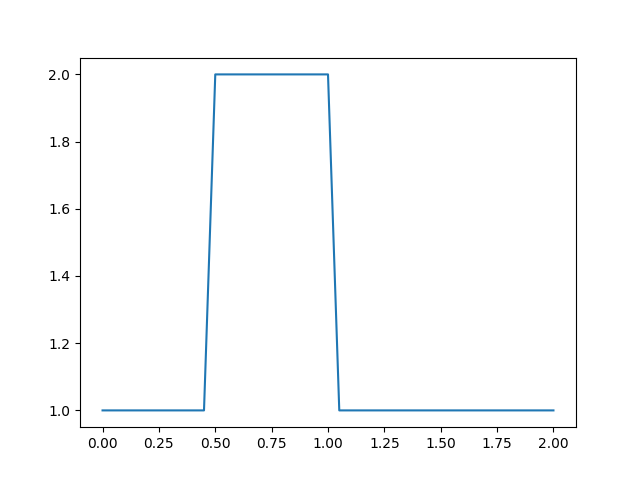
\includegraphics[width=20em]{compscieng_app45cfd1_01.png}

Üstteki bir fonksiyon türü aslında, ona görüntüsü sebebiyle ``şapka fonksiyonu''
ismi de veriliyor.

Şimdi taşınım akımı denkleminin ayrıksal kodlamasına gelelim, burada sonlu
farklılık (finite difference) yaklaşımı kullanıyoruz, $u$ vektörü içindeki her
öge için (1) formülünü işleteceğiz.

\begin{minted}[fontsize=\footnotesize]{python}
un = np.ones(nx)
for n in range(nt):
    un = u.copy() 
    for i in range(1, nx):
        u[i] = un[i] - c * dt / dx * (un[i] - un[i-1])        
\end{minted}

Üstteki işlemle zamanı ileri sardık ve fonksiyon belli bir noktaya geldi. Nereye
geldi?

\begin{minted}[fontsize=\footnotesize]{python}
plt.plot(np.linspace(0, 2, nx), u);
plt.savefig('compscieng_app45cfd1_02.png')
\end{minted}

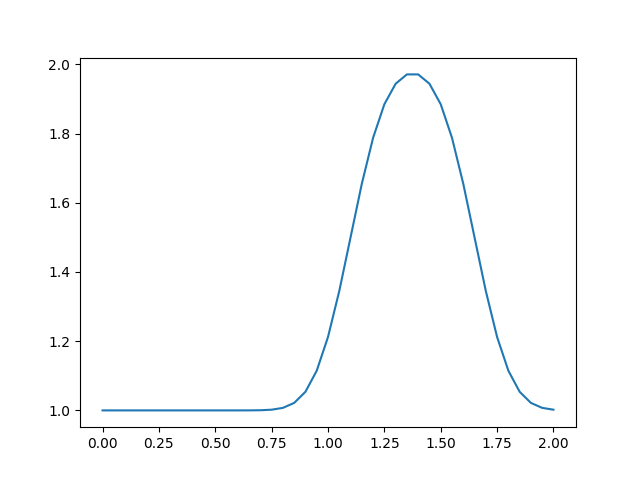
\includegraphics[width=20em]{compscieng_app45cfd1_02.png}

Evet, başlangıç fonksiyonu hakikaten sağa doğru taşındı. Fakat artık fonksiyon
bir şapka değil. Ne oldu? Sonuç yaklaşık temsilin kalitesiyle alakalı, \verb!dx!
ve \verb!dt! küçültüldükçe kalite artacaktır, ve şapkaya daha çok benzeyen
sonuçlar görülecektir. 

Gayrı Lineer Taşınım Akımı (Nonlinear Convection)

Şimdi biraz önceki teknikleri kullanarak gayrı lineer taşınım akımı
kodlayacağız, tek boyutta denklem,

$$
\frac{\partial u}{\partial t} +
u  \frac{\partial u}{\partial c}  = 0
$$

Dikkat edersek önceki denklemdeki $c$ ile çarpım yerine şimdi $u$ ile çarpım
var, bu sebeple formülün ikinci terimi gayrı lineer hale geldi. Eğer
ayrıksallaştırma işlemini tekrar uygularsak, alttaki sonuca erişiriz,

$$
u_i^{n+1} = u_i^n -  u_i^n \frac{\Delta t}{\Delta x} ( u_i^n - u_{i-1}^n )
$$

\begin{minted}[fontsize=\footnotesize]{python}
nx = 41
dx = 2 / (nx - 1)
nt = 20
dt = .025 
u = np.ones(nx)
u[int(.5 / dx) : int(1 / dx + 1)] = 2  
un = np.ones(nx)
\end{minted}

\begin{minted}[fontsize=\footnotesize]{python}
un = np.ones(nx)
for n in range(nt):
    un = u.copy() 
    for i in range(1, nx):
        u[i] = un[i] - un[i] * dt / dx * (un[i] - un[i-1])        
\end{minted}

\begin{minted}[fontsize=\footnotesize]{python}
plt.plot(np.linspace(0, 2, nx), u);
plt.savefig('compscieng_app45cfd1_03.png')
\end{minted}

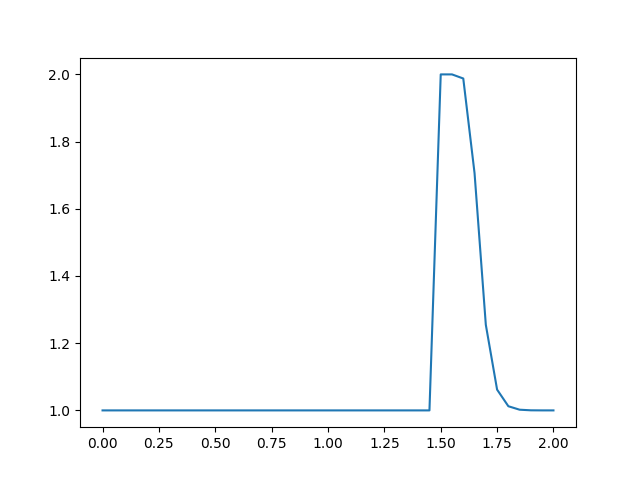
\includegraphics[width=20em]{compscieng_app45cfd1_03.png}

Yakınsama (Convergence)

Lineer taşınım hesabında ortaya çıkan tepe şeklinin ızgara çözünülürlüğü ile
alakalı olduğunu söylemiştik. Bunu birkaç farklı çözünürlük ile deneyerek
görelim. İlk gördüğümüz sonuç \verb!nx=41! kullandı. Arttıralım,

\begin{minted}[fontsize=\footnotesize]{python}
def linearconv(nx):
    dx = 2 / (nx - 1)
    nt = 20    
    dt = .025  
    c = 1

    u = np.ones(nx)
    u[int(.5/dx):int(1 / dx + 1)] = 2  

    un = np.ones(nx)

    for n in range(nt):
        un = u.copy() 
        for i in range(1, nx):
            u[i] = un[i] - c * dt / dx * (un[i] - un[i-1])
        
    plt.plot(np.linspace(0, 2, nx), u);

linearconv(61)
plt.savefig('compscieng_app45cfd1_04.png')
\end{minted}

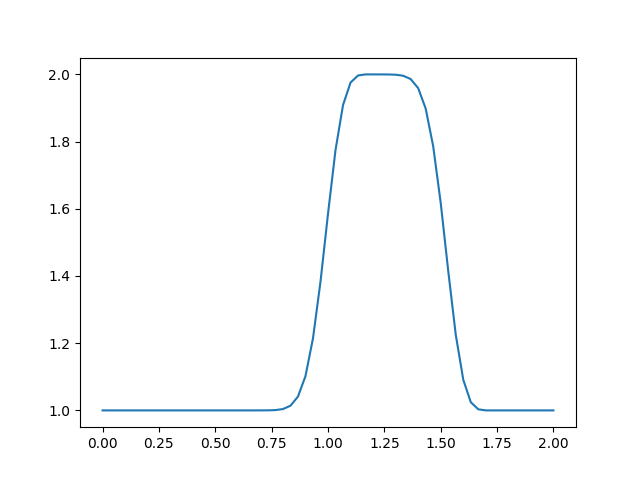
\includegraphics[width=20em]{compscieng_app45cfd1_04.png}

\begin{minted}[fontsize=\footnotesize]{python}
linearconv(71)
plt.savefig('compscieng_app45cfd1_05.png')
\end{minted}

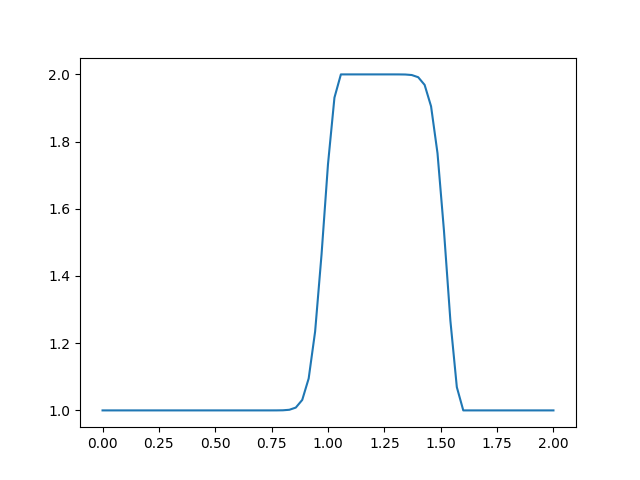
\includegraphics[width=20em]{compscieng_app45cfd1_05.png}

Gittikçe daha fazla şapka fonsiyonuna benzer sonuçlar alıyoruz. Şimdi dikkat,
bir kez daha arttıralım,

\begin{minted}[fontsize=\footnotesize]{python}
linearconv(85)
plt.savefig('compscieng_app45cfd1_06.png')
\end{minted}

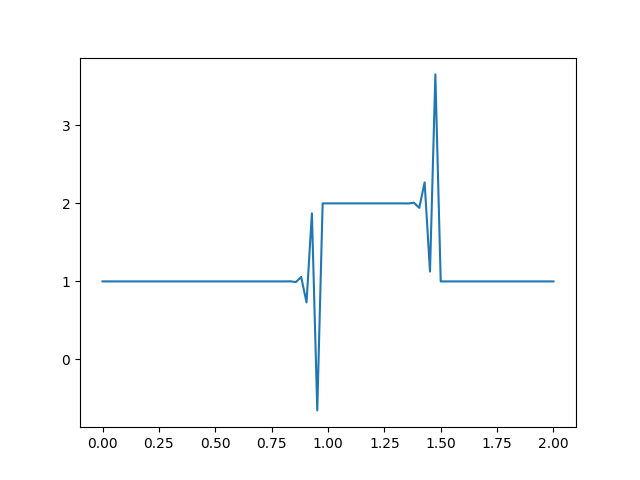
\includegraphics[width=20em]{compscieng_app45cfd1_06.png}

Bu sonuc sapka fonksiyonuna benzemiyor. Ne oldu?

Hesaplananları düşünürsek, yer ekseni üzerinde dalganın hareketini hesaplıyoruz,
fakat her adımda $\Delta t = 0.025$ farzederk bu hesapları yapıyoruz. Üstteki
yanlış sonuçta $\Delta t$ zaman aralığında öyle bir adım attık ki bu adım
\verb!dx!'in büyüklüğünden daha fazla. Bu durum ilk denemelerde ortaya çıkmadı
çünkü \verb!dx! yeterince büyük tutulmuştu. Fakat onu küçültükçe bir noktada
hesap patladı. 

Kaynaklar

[1] Barba, {\em 12 steps to Navier–Stokes, Ders 1},
    \url{https://nbviewer.jupyter.org/github/barbagroup/CFDPython/blob/master/lessons/01_Step_1.ipynb}

[2] Bayramlı, {\em Kısmi Türevsel Denklemler, Dalga Denklemini Türetmek}

[3] Saad, {\em CH EN 6355 – Computational Fluid Dynamics},
    \url{http://www.tonysaad.net/ucfd/}

\end{document}


